\documentclass[a4paper]{article}
\usepackage{amsmath,amssymb,caption,float,graphicx,xcolor}
\usepackage{minted}
\usepackage[utf8]{inputenc}
\usepackage[english]{babel}
\usepackage[backend=bibtex]{biblatex}
\addbibresource{Lab4.bib}
\captionsetup[figure]{labelsep=period}
% \captionsetup[table]{labelsep=period}
\definecolor{bg}{rgb}{0.95,0.95,0.95}
\renewcommand\thesection{\arabic{section}}
\usemintedstyle{emacs}
\begin{document}
\begin{center}
    \huge
    \textbf{ECE4730J\\Advanced Embedded System\\}
    \LARGE
    \vspace{15pt}
    \textsc{Lab 4: Write and Load a Kernel Module}\\
    \large
    \vspace{5pt}\today\\
    \vspace{5pt}
    \begin{tabular}{ll}
        Name&Student ID\\
        Yihua Liu&518021910998\\
        Shuocheng Chen&517021911139\\
        Yiming Ju&518370910059\\
    \end{tabular}
    \vspace{5pt}
    \rule[-5pt]{.97\linewidth}{0.05em}
\end{center}
1. \texttt{Bash} script \cite{compilingkm}:
\begin{minted}[frame=single,bgcolor=bg,breaklines,linenos]{bash}
mkdir modules
cd modules
# Copy simple_module.c to modules by SFTP/SCP
# Write a Makefile
sudo apt install bison  # dependency
sudo make -C /usr/src/linux-headers-5.11.0-1021-raspi M=$PWD modules
\end{minted}
\texttt{Makefile} \cite{love2010linux}:
\begin{minted}[frame=single,bgcolor=bg,breaklines,linenos]{makefile}
obj-m := simple_module.o    
\end{minted}
Note that \texttt{SUBDIR=} is no longer supported since Ubuntu 20.04, use \texttt{M=} instead \cite{subdir}. Detailed information is summarized in \cite{classmap}. Output:
\begin{minted}[frame=single,bgcolor=bg,breaklines,linenos]{text}
make: Entering directory '/usr/src/linux-headers-5.11.0-1021-raspi'
CC [M]  /home/yihua/modules/simple_module.o
MODPOST /home/yihua/modules/Module.symvers
CC [M]  /home/yihua/modules/simple_module.mod.o
LD [M]  /home/yihua/modules/simple_module.ko
make: Leaving directory '/usr/src/linux-headers-5.11.0-1021-raspi'      
\end{minted}
It will generate:
\begin{itemize}
    \item Module.symvers
    \item modules.order
    \item simple\_module.ko
    \item simple\_module.mod
    \item simple\_module.mod.c
    \item simple\_module.mod.o
    \item simple\_module.o
    \item .Module\_symvers.cmd
    \item .modules.order.cmd
    \item .simple\_module.ko.cmd
    \item .simple\_module.mod.cmd
    \item .simple\_module.mod.o.cmd
    \item .simple\_module.o.cmd
\end{itemize}
\begin{figure}[H]
    \centering
    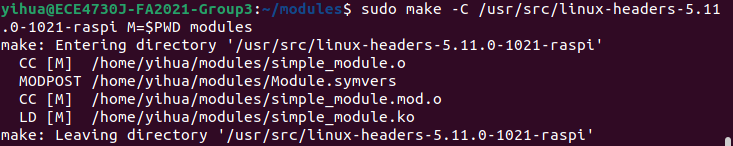
\includegraphics[width=1\textwidth]{1.png}
    \caption{The output after we compile the module.}
\end{figure}
2. Output of \texttt{dmesg}:
\begin{minted}[frame=single,bgcolor=bg,breaklines,linenos]{text}
[11933.762154] simple_module: loading out-of-tree module taints kernel.
[11933.762612] simple_module initialized
\end{minted}
\begin{figure}[H]
    \centering
    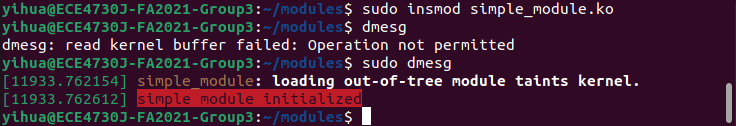
\includegraphics[width=1\textwidth]{2.png}
    \caption{The message that appears in the system log.}
\end{figure}
3. Output of \texttt{lsmod} \footnote{Warning: do not use \texttt{Lab4-*.log} for the file names of $\backslash$ inputminted, otherwise they will be deleted by \texttt{bibtex}.}:
\inputminted[frame=single,bgcolor=bg,breaklines,breakanywhere,linenos]{text}{Lab4-3.txt}
\begin{figure}[H]
    \centering
    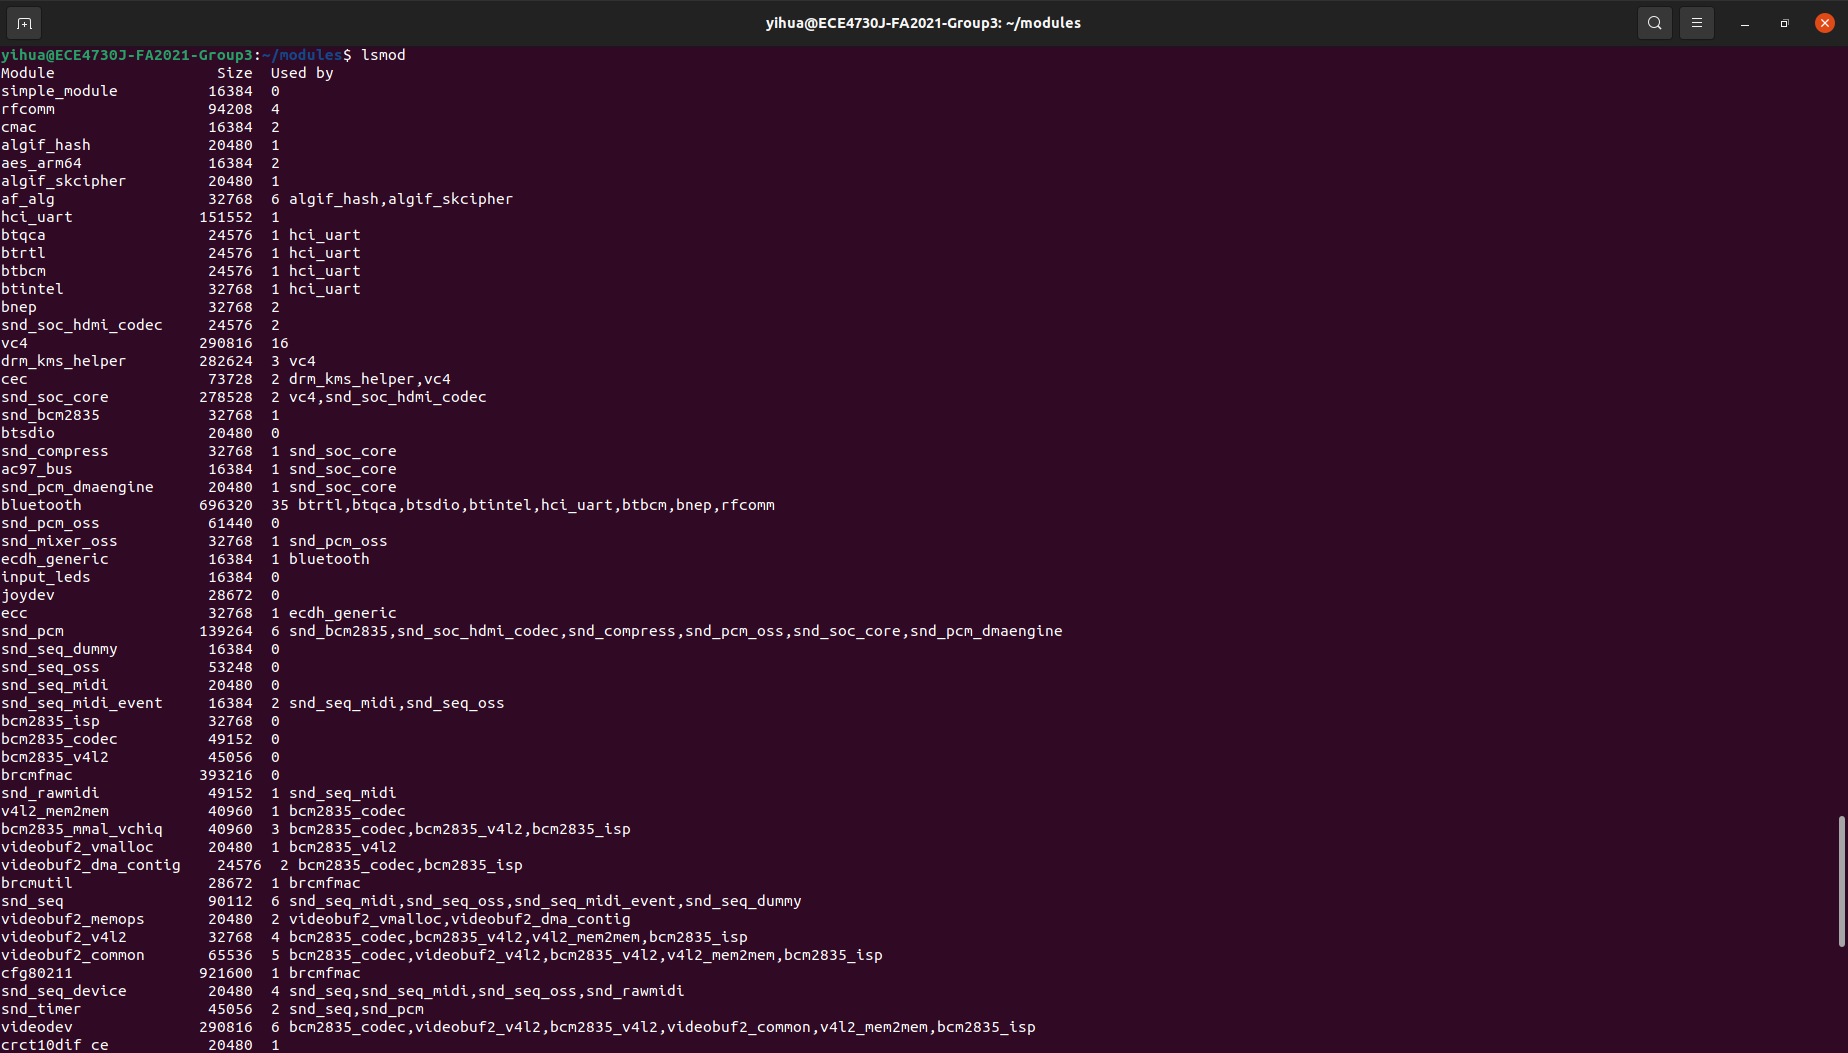
\includegraphics[width=1\textwidth]{3.png}
    \caption{The output that was produced by \texttt{lsmod}.}
\end{figure}
4. Output of \texttt{lsmod}:
\inputminted[frame=single,bgcolor=bg,breaklines,breakanywhere,linenos]{text}{Lab4-4.txt}
\begin{figure}[H]
    \centering
    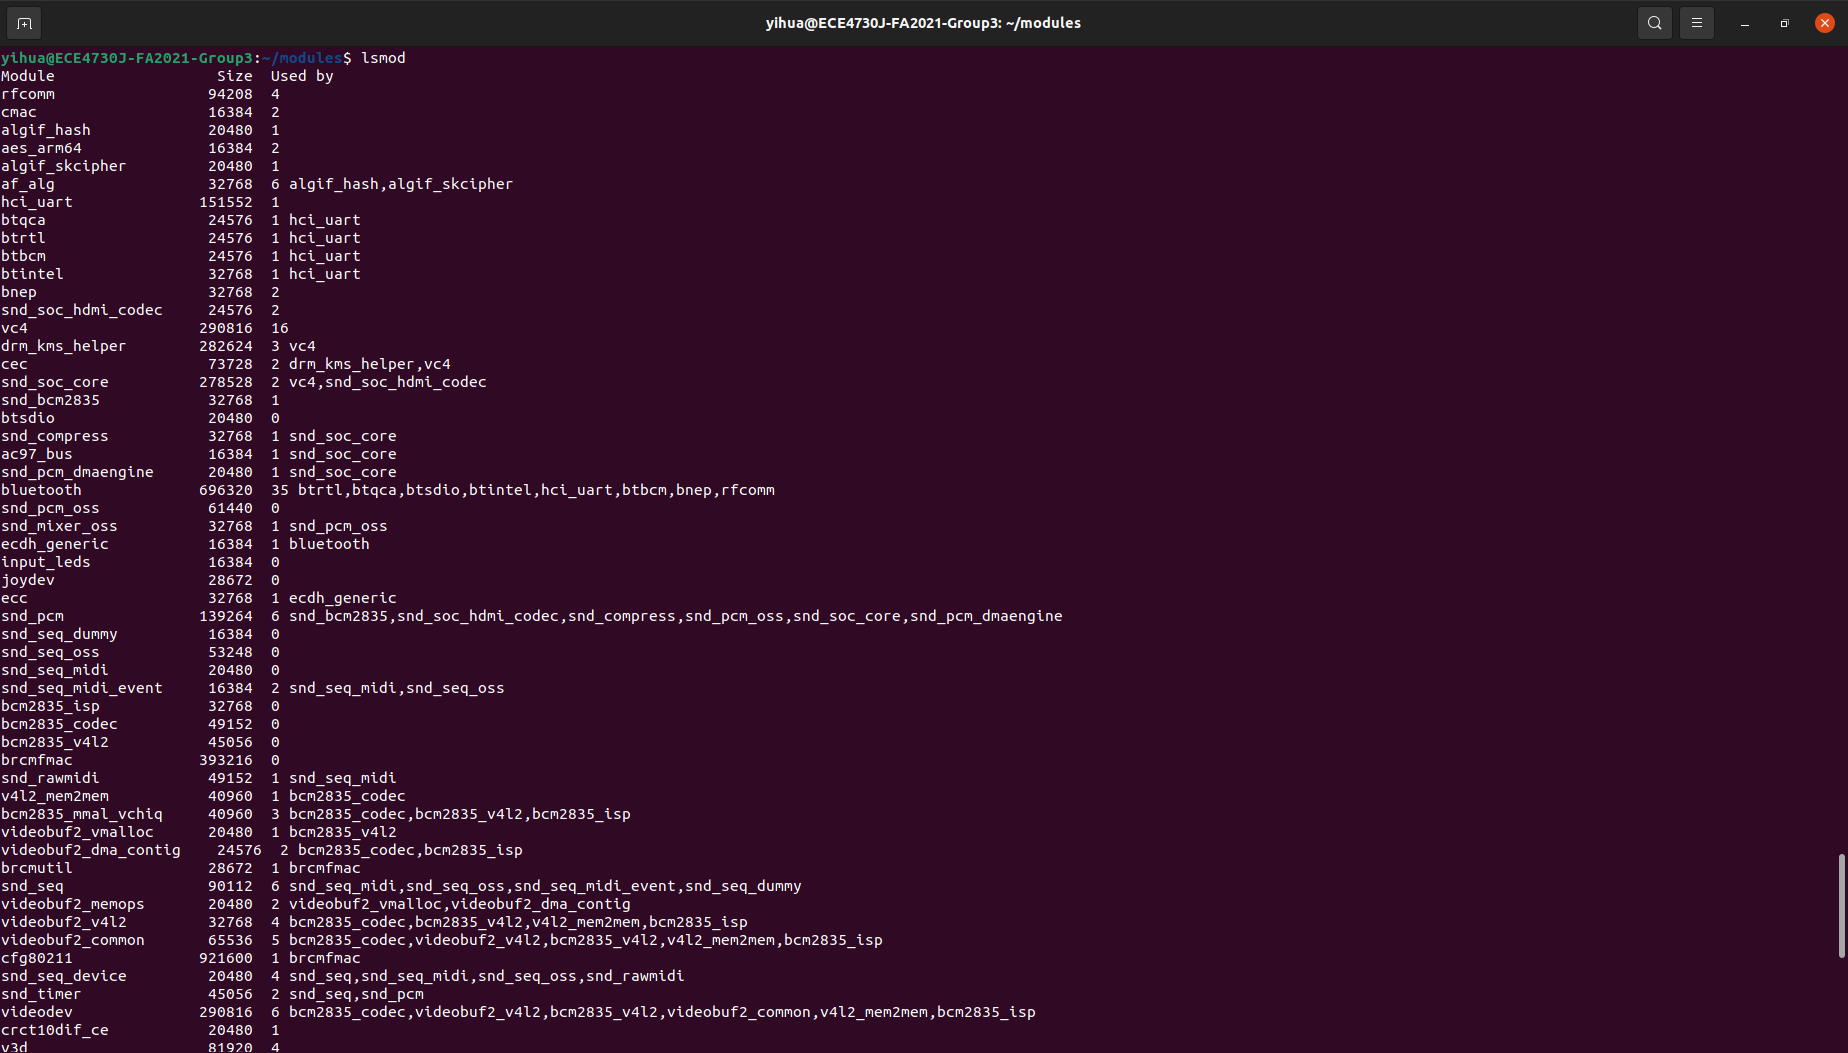
\includegraphics[width=1\textwidth]{4.png}
    \caption{The output of \texttt{lsmod}.}
\end{figure}
Output of \texttt{dmesg}:
\begin{minted}[frame=single,bgcolor=bg,breaklines,linenos]{text}
[11933.762154] simple_module: loading out-of-tree module taints kernel.
[11933.762612] simple_module initialized
[12616.534349] simple_module is being unloaded
\end{minted}
\begin{figure}[H]
    \centering
    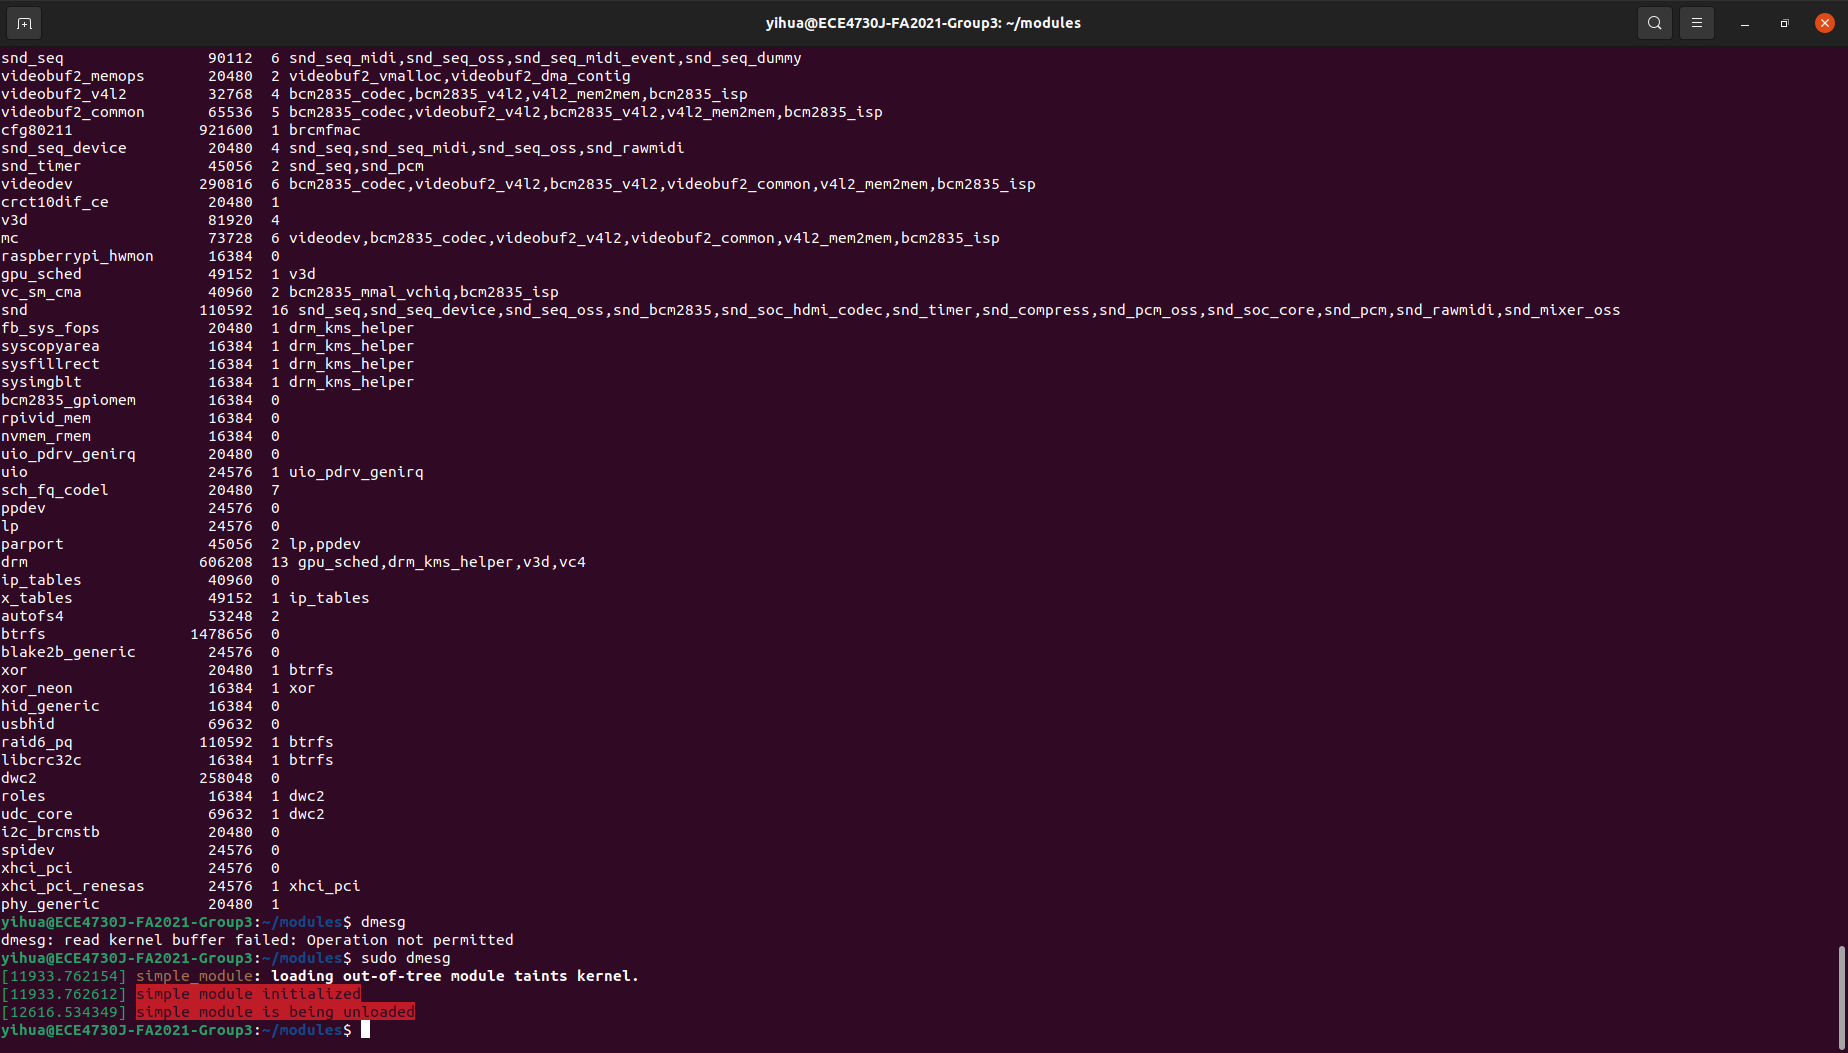
\includegraphics[width=1\textwidth]{5.png}
    \caption{The line of the system log, which show that the module was unloaded.}
\end{figure}
5. \texttt{Bash} script:
\begin{minted}[frame=single,bgcolor=bg,breaklines,linenos]{bash}
sudo make -C /usr/src/linux-headers-5.11.0-1021-raspi M=$PWD modules
sudo dmesg --clear
sudo insmod jiffies.ko
sudo dmesg
sudo rmmod jiffies.ko
sudo dmesg
\end{minted}
\texttt{Makefile}:
\begin{minted}[frame=single,bgcolor=bg,breaklines,linenos]{makefile}
obj-m := jiffies.o
\end{minted}
\begin{figure}[H]
    \centering
    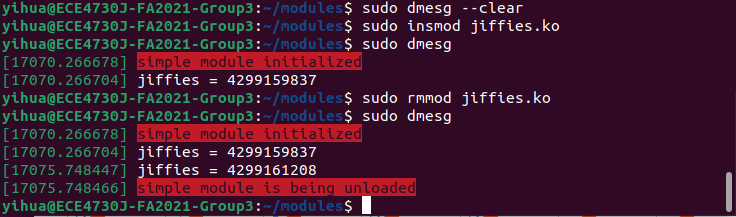
\includegraphics[width=1\textwidth]{6.png}
    \caption{The system log message that shows the values of the jiffies variable when the module was loaded and unloaded.}
\end{figure}
Source code \cite{jiffies}:
\inputminted[frame=single,bgcolor=bg,breaklines,linenos]{c}{modules/jiffies.c}
\printbibliography
\end{document}